\hspace{6.5cm}

% \begin{wrapfigure}{r}{0.4\linewidth}
%   \begin{minipage}[h]{\linewidth}
%     \musicannot{Repetition Repeats all other Repetitions\\\emph{for 10-stringed guitar and computer}\\Composed \& premiered in 1996 \\Commissioned by and dedicated to Stefan \"{O}stersj\"{o}}
%   \end{minipage}
% \end{wrapfigure}

\begin{wrapfigure}{r}{0.45\linewidth}
  \begin{minipage}[h]{\linewidth}
    \begin{flushright}
      \musicannot{Repetition Repeats all other Repetitions\\
        \emph{for ten-stringed guitar and computer}\\
        Composed \& premiered in 2006\\
        Commissioned by and dedicated to Stefan \"{O}stersj\"{o}}
    \end{flushright}
  \end{minipage}
\end{wrapfigure}

%%% Local Variables: 
%%% mode: latex
%%% TeX-master: "../ImprovisationComputersInteraction"
%%% End: 


% \vspace{1cm}
\noindent In this chapter the work-in-movement \emph{Repetition Repeats all other Repetitions} and the context from which it came into being are discussed. Although the text here summarises the two essays \citetitle{frisk-ost06} and \citetitle{frisk-ost06-2} some of the thinking here depends on those texts. Just as those two essays were co-written with Stefan \"{O}stersj\"{o}, the guitarist who commissioned \emph{Repetition}, the current chapter is largely based on a co-written text.\footcite[Another version of the original text is part of his PhD thesis. See][]{ostersjo08} Owing to the collaborative nature of the project, and to avoid tedious repetitions, throughout the text I refer to Stefan by his first name only and when I use `we' and `us' I consistently refer to Stefan and me. The primary purpose of the studies within \emph{Negotiating the Musical Work}\footnote{See \fullcite{frisk-ost06}; and \fullcite{frisk-ost06-2}} was to understand musical collaboration and composer-performer interaction better but already in the first study it became clear to us that much of the knowledge could equally well be used in terms of musician-computer interaction, which, to me, was emerging as the more interesting aspect of these studies. These ideas contributed strongly to the emergence of the idea of \index{interaction!as difference}\index{interaction-as-difference}interaction-as-difference as well as the giving up of the \index{Self}Self.


In order to unwrap the processes that led to the first version of \emph{Repetition Repeats all other   Repetitions}\footnote{Henceforth referred to as \emph{Repetition}.} and eventually to the expanded concept of the `open work', it should be clear that many circumstances, some of which are auxiliary to the actual process of 'composing' (i.e. the tasks traditionally assigned to the `composer') had a great influence on the way the piece developed. In the end, however, it turned out that these 'circumstances' or 'processes' were not in fact 'auxiliary': They were, or would become, an integral part of the process of composing (now also in the extended sense of the term). Some of these were planned and others came about as a result of the ways in which the project developed. For example, one of the outspoken intentions was to use \emph{Repetition} as a testbed for my timbre tracking \index{software}software \emph{timbreMap} (see \ref{sec:timbremap}), and one of the perhaps more unexpected consequences was the formation of a new group, \emph{\useGlosentry{glos:six-tones}{The Six Tones}}, which can be seen as a direct consequence of the collaboration Stefan and I had initiated in January 2006. Not only an offspring of our collaboration \emph{The Six Tones}, as is often the case with multi-project collaborations, also provided important material for \emph{Repetition}. A timeline of some of the more important events relating to this project may be gathered from Figure \ref{fig:repetition-timeline}, and below I give an account of the development of the piece---and the development of the project---and the circumstances that, according to my own biased view, were the most important ones to shape the piece (i.e. most important with regard to the theme of this book). It should, however, be clear to the reader that the process of composing, or constructing, \emph{Repetition} has not yet come to an end, but continues to feed material and events into the `container' that \emph{Repetition} has come to represent. In its first conception, although the \emph{project} was thought of as collaborative, the \emph{music itself}---the score and its performances---was not. But the stream of events born out of the process shaped \emph{Repetition} as a truly collaborative effort, in which the members of the collaboration were no longer limited to myself and Stefan \"{O}stersj\"{o} and me. Some of these events are described in the following sections and may be summarised as:

\begin{enumerate}[(1)]
\item \textbf{Negotiating the Musical Work} That Stefan \"{O}stersj\"{o} and I had mutually agreed on \emph{Repetition} being part of my own, as well as his, doctoral research project is an important factor that, in the end, greatly influenced the result. In particular the preparatory studies and the papers we wrote as a result had impact on the development of the project.% %$|$\hyperref[sec:negotiating-1]{here}
%
\item \textbf{The Six Tones}\footnote{As is more fully explained in Section \ref{sec:negotiating-2} \emph{The Six Tones} was composed for a newly formed Vietnamese-Swedish quartet that later takes its name from the title of the composition \emph{The Six Tones}.} Working with \emph{The Six Tones} added other kinds of instrumental and sonic input and it intensified the social aspect of our collaboration owing to the additional work relation. There is also a close intertextual relation between my piece \emph{The Six Tones} and  \emph{Repetition} in that each contains transcriptions of the other. %$|$  \hyperref[sec:negotiating-2]{here}
%
\item \textbf{The first version} A combination of events, decisions and circumstances led to the decision \emph{not} to employ `true' interactivity in the first version performed in October 2006. This radical conclusion gave birth to the idea of \emph{Repetition} as a piece that can have many independent instances.% $|$  \hyperref[sec:negotiating-3]{here}
%
\item \textbf{Symphonie Diagonale} The next version would be even less \emph{\index{real-time}\index{time!real-time}real-time} interactive and even \emph{more} collaborative and this time had already been performed a number of times. %$|$\hyperref[sec:negotiating-4]{here}
%
\item \textbf{The annotated score} Although primarily concerned with `preservation' (see the section on \hyperlink{sec:target:libintegra-1}{libIntegra in the Introduction}), working with the Integra project\footnote{See \url{http://www.integralive.org} and \cite{frisk-bull07,frisk-bullock08}.} made me start thinking of a representation of the \index{ontology}ontology of a musical work as a possibility for a documentation of the `work in motion'; this being the kind of work with which Stefan and I would associate \emph{Repetition}.% $|$  \hyperref[sec:negotiating-6]{here} 
\end{enumerate}

\begin{figure}[htb]
  \centering
  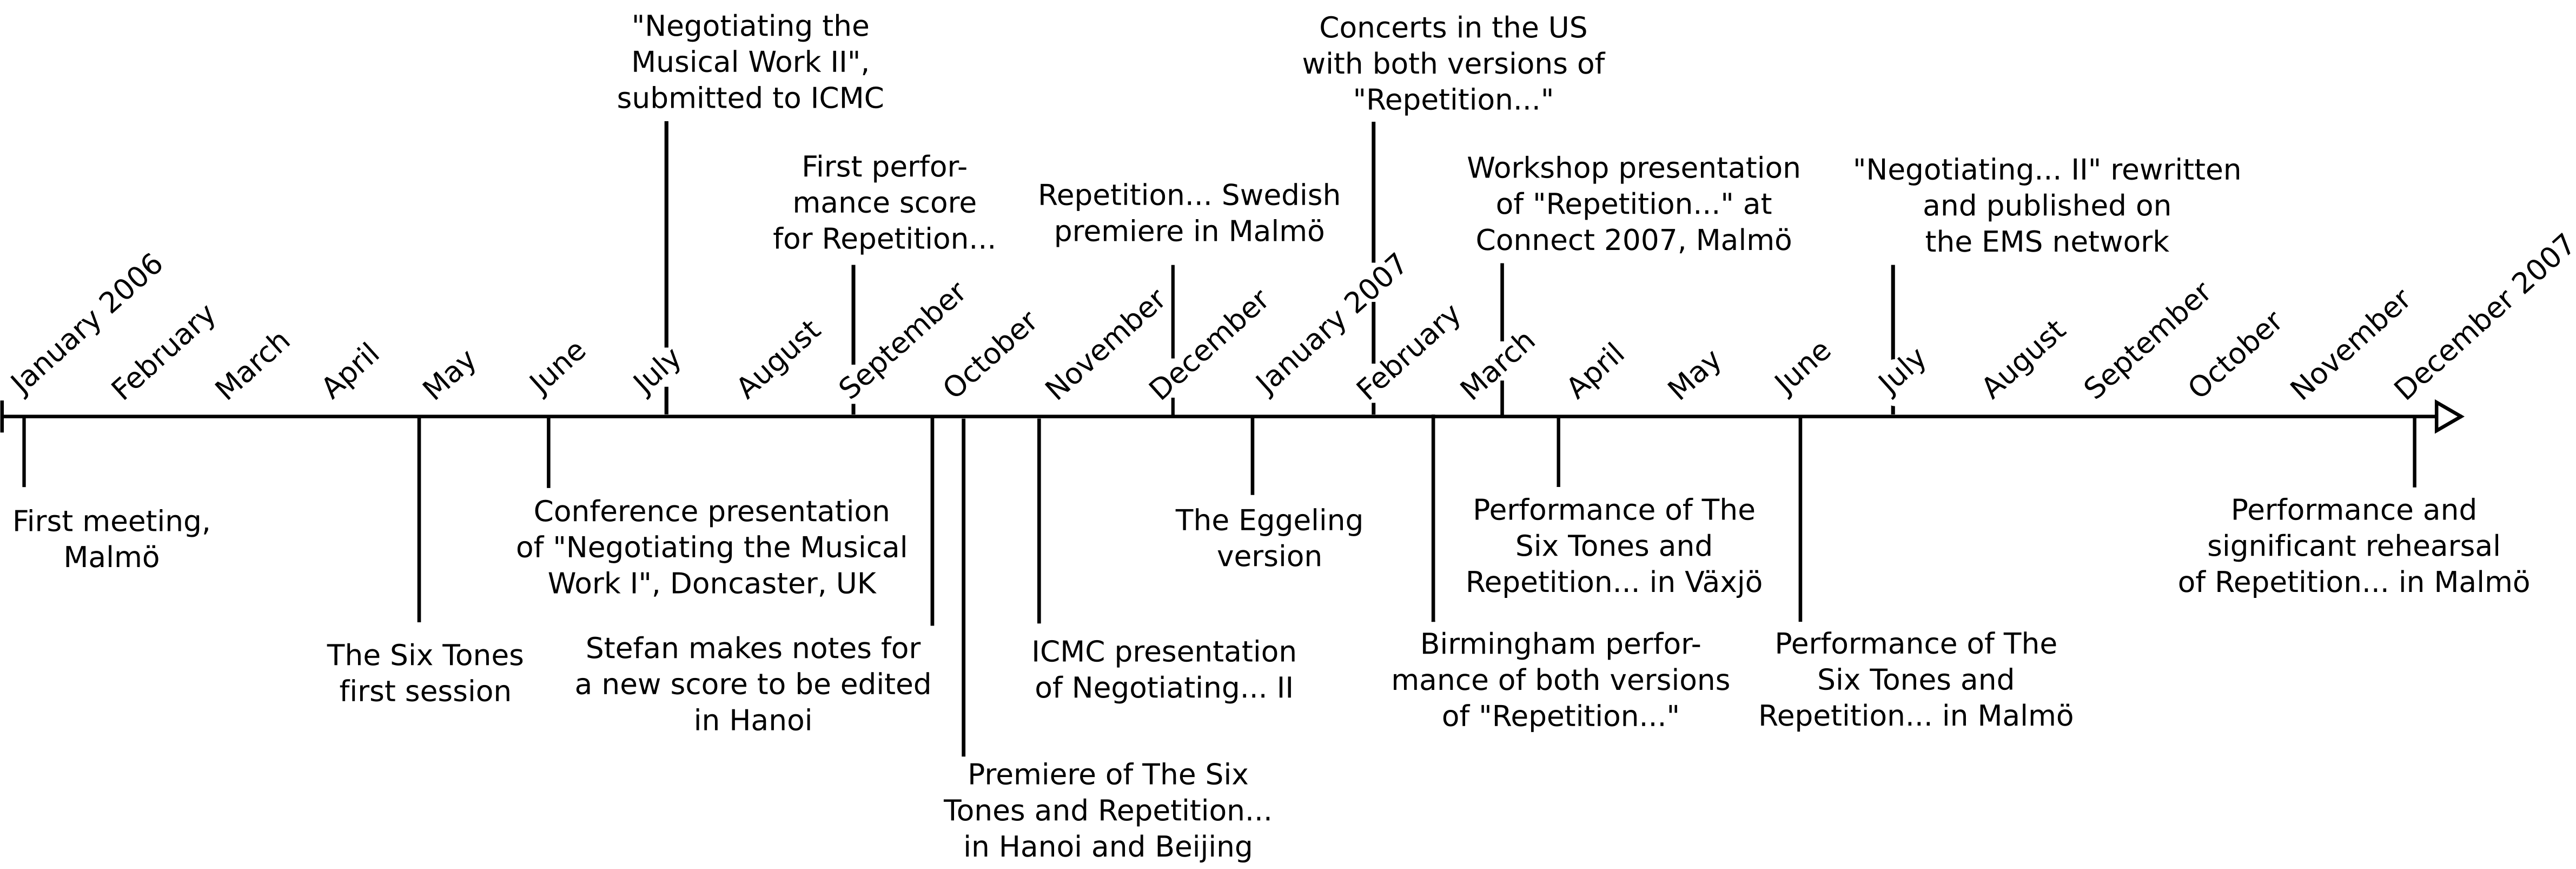
\includegraphics[width=\textwidth]{img/Repetition-timeline}
  \caption[Time line of events relating to \emph{Repetition\ldots}]{The events mapped on a time line relating to the life span of \emph{Repetition Repeats all other Repetitions}.}
  \label{fig:repetition-timeline}
\end{figure}

%\marginpar{\listoftags{\tagword{Repetition}, \tagword{timbreMap},
%\tagword{Negotiate}, \tagword{Semiology} }}

\section{Observing negotiations of the musical work}
\label{sec:negotiating-1}

\begin{wrapfigure}{r}{0.4\linewidth}
  \begin{minipage}[h]{\linewidth}
    \begin{flushright}
      \musicannot{Negotiating the Musical Work\\
        \emph{video analysis of a composer-performer session}}
      \end{flushright}
  \end{minipage}
\end{wrapfigure}

%%% Local Variables: 
%%% mode: latex
%%% TeX-master: "../ImprovisationComputersInteraction"
%%% End: 

Part of our agreement, and perhaps a first prerequisite for any successful composer-musician collaboration, was the idea of partly giving up the traditional view of our respective roles.\footnote{This process belongs to the notion of giving up the \index{Self}Self.} We would each allow ourselves to enter the domain of the other and we would allow each allow the other to enter our own professional sphere. In one of the earliest results of this project---the documentation of a study of a collaboration similar to ours, between Stefan \"{O}stersj\"{o} and Swedish composer Love Mangs---we had seen an example of this behaviour.\footcite{frisk-ost06} In the analysis of the video documentation of their collaboration, from which we had chosen a few excerpts, there were moments when Mangs was giving input to the process ``as if'' he was interpreting the material and moments when Stefan was manipulating the material ``as if'' he was the composer. I say ``as if'', because although the project was an outspoken collaboration in which the two musicians would meet and work out the material together, it is noted in the analysis that  Love Mangs in particular was not entirely comfortable with the floating nature of his identity as composer.

In the study \emph{Negotiating the Musical Work}, in an attempt to build an experimental framework to be used to unwrap these processes, we discuss the semiological model for musical analysis by musicologists Jean-Jacques Nattiez and Jean Molino. Their model looks at the work of art as an object that may be analysed from three different perspectives or levels: ``the poietic, the esthesic and the `neutral''.\footcite{molino} Three modes all representing the same work of art where the \useGlosentry{glos:poietic}{poietic} level is the constructive phase, the \useGlosentry{glos:esthesic}{esthesic} is the interpretative phase and the neutral is the trace left by the poietic (or esthesic) process\footcite{molino}\nocite{molino2}. At the time, this tripartite model was the object of some excitement to Nattiez, who believed that 
%%
\begin{squote}
[\ldots] recognizing, elaborating, and articulating the three relatively autonomous levels (\useGlosentry{glos:poietic}{poietic}, neutral and \useGlosentry{glos:esthesic}{esthesic}) facilitates knowledge of all processes unleashed by the musical work, from the moment of the work's conception, passing through its `writing down', to its performance. \footcite{nattiez}
\end{squote}
%%

\label{sec:1-par:2}
For perhaps obvious reasons the musical semiology proposed by Nattiez has been criticised and discussed widely, and it is not my intention to engage in that somewhat dated debate here.\footnote{The   concept of the `neutral analysis' or `analysis on the neutral level'   is particularly troublesome. For an insight in the debate from both   sides, see \cite{nat89} and \cite{dunsby83}.} Nevertheless, the terminology of Nattiez and Molino proved to be useful to us. Our adaptation of it, in particular the two levels \emph{poietic} and \emph{esthesic}, helped us reconsider the traditional division of labor between `musician' and `composer'. Whereas Nattiez lean on semiology in order to confirm the authority of the composer as the creator of the work (with the interpreter `inserted' towards the end of the poietic process\footcite[See][73]{nattiez}), we used it to depict what we analysed as a rather rapid oscillation between poietic and esthesic processes, and whereas Nattiez in his book \citetitle{nattiez} is primarily concerned with the composed \emph{work} and its \index{ontology}ontology, we focused on the interactions involved in the phases \emph{prior} to the existence of a score and prior to the first performances. The process of writing down a musical work, we argue, is not a unidirectional poietic process, but is described by us as an \emph{interaction} between esthesic and poietic processes, to an extent that makes it difficult to define the end of one and the beginning of the other. What Stefan and I attempted to show in the studies mentioned above is that the acts of musical composition that Nattiez gathers within the poietics can in themselves be analysed by using the same method that he applies to the total fact of the musical work. Nattiez seems to be drawing conclusions about ``processes unleashed by the musical work'' from a purely analytical understanding of music, from a perspective still dependent on the view of composers as `true creators' and works as `ideal objects' (in the phenomenological sense); stable and fixed artworks that should make up the primary object of study for musicology. What we were concerned with then, and what I am concerned with here, is almost the opposite: at least we are operating on the other side of the dividing line constituted by the completed score, the musical work as a coherent object, namely prior to the existence of a score and prior to the performance. Our concern is to attempt to understand the actions that \emph{lead to} musical content and the significance of the interactions between the agents involved in these processes, and to investigate the meaning of collaboration in the musical \emph{poesis} and the significance of these processes with regard to the technological \emph{poesis} in musician-computer interactivity.

% \floatstyle{plain}
% \newfloat{Reflection}{H}{lop}[section]
% \begin{Reflection}
% \end{Reflection}

% Just as we found in our  study is there no such thing as 'only right % hemisphere' in  composing or improvising or programming. Nor does a % concept such  as 'inspiration' pertain to one hemisphere only. 

% Becoming: becoming saxophone, becoming computer 
% In the actual saxophone there is something of all the other things % that can become improvisation. That something is the virtual side.

\label{sec:1-par:3}
In Figure \ref{fig:timeline-mangs} we plot our analysis of the interaction between Stefan and Love Mangs. The activities (utterances, expressions, topics, etc.) are summarised by the white squares and the horizontal position of the squares shows who initiated the activity (Stefan on the right and Love on the left) and the mode (esthesic or poietic) with which we coupled it. The arrows pointing to and from the activity squares show the directionality of the communication and in the middle is an initiative curve, i.e. which of the two musicians holds the initiative at a given moment. Dashed lines in the communication arrows indicate a `noisy' or `dropped' message; a message that was misunderstood or not picked up by the other party. It should be noted that the graph is obviously a rough generalisation: the actual interaction between Stefan and Love Mangs was not so tidily square. Nevertheless, the graph shows an example of the non-linear and flexible character of their communication. From looking at the graph we can see that during this clip there is a tendency towards communicative clarity. At the top of the graph there is what seems to be a fair amount of confusion, a lot of individual activity not responded to (as is represented by the dashed lines of communication). Towards the bottom of the graph, however, the interaction is denser and appears to be less noisy, with the result that fewer messages are lost. In addition, as the composer in this session, Love Mangs is moving from being active almost exclusively in the esthesic domain to operating mainly in the poietic domain.\footnote{The analysis of the graph in Figure \ref{fig:timeline-mangs}---and of the events preceding it--- should only be seen as a summary. For a more complete and detailed discussion of the \"{O}stersj\"{o}/Mangs collaboration in general, see \cite[Chap.~3]{ostersjo08} and for a more in-depth analysis of the video clip discussed above see \cite[Sec.~3.2]{frisk-ost06} and \cite[Sec.~4]{frisk-ost06-2}.}

\label{sec:1-par:4}

The miscommunication, or rather the \emph{negotiation}, observable in the beginning of the session appears to play the role of a `tuning-in' between the two agents (see \hyperref[sec:timbremap]{Section \ref*{sec:timbremap}}), a tuning-in through negotiation that, towards the end of the session, allows the relations to become established in a way that permits creative decisions. One of the suggestions we make in \citetitle{frisk-ost06-2} is that Stefan and Love Mangs, in their negotiations, are defining a \emph{subculture}, against which the symbols \hyperref[fig:timeline-mangs]{in the graph} which represent ideas exchanged (e.g. the \emph{fermata} starting at line 45-65 or the \emph{arpeggio} roughly at line 145) derive their meaning. These thoughts lead us back to semiological thinking, though in a more general sense than that proposed by \citeauthor{nattiez} and \citeauthor{molino}. Umberto Eco claims that ``[a]ny attempt to establish the referent of a sign will force us to define this referent with the terminology of an abstract entity''.\footcite[66]{eco71} The signs, according to Eco, denote cultural entities which remain unaltered when the sign is transposed or translated. In this case, however, it is the abstract entity that is transposed in order to reveal the meaning of the symbol within this specific context. The \emph{fermata} in the example may or may not be related to the romantic idea of a fermata. Furthermore, there is likely to be a significance attached to the symbol that evades its immediate `meaning'. Both Stefan and Love Mangs are working within the frame of their own cultural contexts which define their respective understandings of the evolving work. The subculture, according to us, is a result of the interaction, and the negotiation (`\emph{What is it we are  developing?}', `\emph{How are we talking about it?}' etc.), between the two agents and their inherent cultural contexts. Their mutual expectations and their understanding or imagination of the work in progress is of importance when they attempt to co-ordinate their actions, for instance, towards a definition of the performance instructions. Where often the composer-performer relation is understood as a hierarchic structure in which the role, even the purpose, of the performer is to fulfil the composer's intentions, this mode of analysis allows us to look at the two agents (composer and performer) as part of a larger system that may also contain many other agents such as social and cultural context, instruments, status, power, gender, etc.

\label{sec:1-par:5}
To summarise the analysis of the Stefan and Love Mangs collaboration, it appears as if the noisy communication early on in the process did not halt the creativity. Ideas, including those that originated in these early and seemingly confusing negotiations, continued to develop while the agents involved slowly established a common space, a subcultural context. Against this context the symbols exchanged were given meaning, or \emph{new} meaning, in every respect different from the traditional meaning of the symbol. Assuming this analysis is correct---that noisy communication is not an obstacle to the establishment of common ground between communicating and collaborating agents---what does it mean to our understanding of computer-musician interaction in the context of \index{electro-acoustic music}electro-acoustic music? There is a tendency, not only in musician-\index{interaction!computer}computer interaction, but in \index{interaction!human-computer}\index{HCI}human-\index{interaction!computer}computer interaction in general, to look at the communication as primarily a one-way stream, in which noise in the transmission is a great problem. From the bottom up the computer is truly \index{digital}digital and it may be correct to let the input to such a system be binary. Looking at it, however, as an agent in a communicative system where binary distinctions are difficult to make and where the communication will be defined in the course of action, so to speak, will certainly present problems. Nevertheless, the study summarised above, and the results we reached in it, became the inspiration for the interactive model used in \emph{Repetition}.

% \begin{wrapfigure}{r}{10cm}
   \begin{figure}[ht]
    \begin{center}
       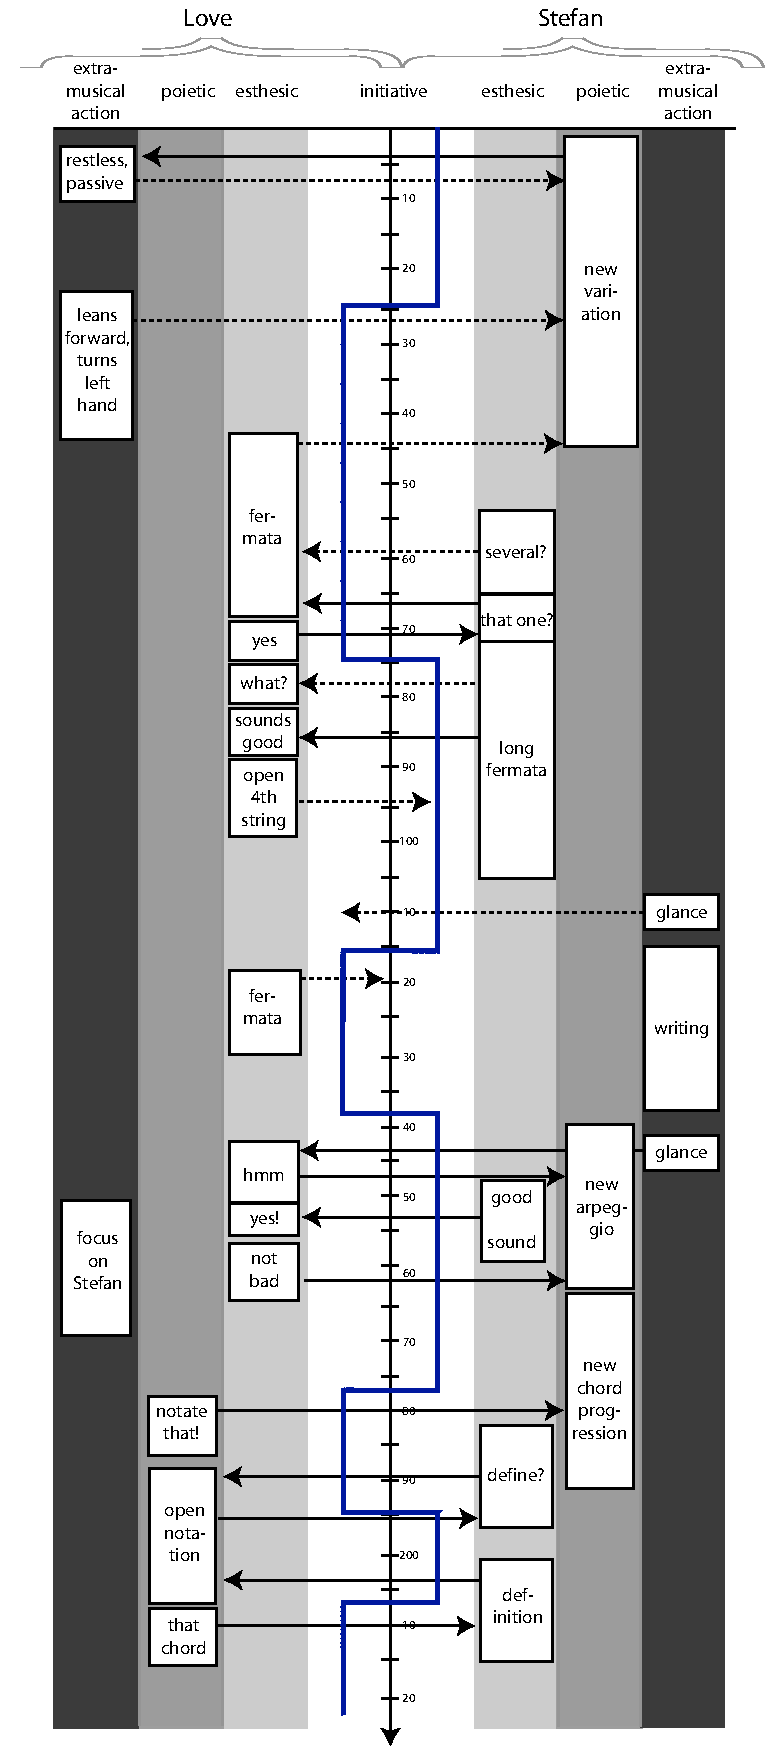
\includegraphics[height=0.85\textheight]{img/timeline_horiz}
    \end{center}
    \caption[A graph of the interaction between Stefan \"{O}stersj\"{o} and Love Mangs.]{A graph of the interaction between Stefan \"{O}stersj\"{o} and Love Mangs in the session analysed and discussed in Section \ref{sec:1-par:3}. The scale in the centre axis refers to line numbers in the transcription of the video and does \emph{not} represent linear time.}
    \label{fig:timeline-mangs}
   \end{figure}
% \end{wrapfigure}


\section{The Six Tones}
\label{sec:negotiating-2}

% \begin{wrapfigure}{r}{0.4\linewidth}
%   \begin{minipage}[h]{\linewidth}
%     \musicannot{The Six Tones\\\emph{for Dan Bau, Dan Tranh, % 10-stringed guitar, banjo and computer}\\Composed \& premiered in % 1996}
%   \end{minipage}
% \end{wrapfigure}
Another factor to consider while tapping into this process---the
process of constructing \emph{Repetition}---is the connection between \emph{Repetition} and a similar, but slightly larger, collaboration performed within the project \emph{The Six Tones}\footnote{As was explained above, the group \emph{The Six Tones} takes its name from the composition of the same name.} whose coming into existence is very closely related to \emph{Repetition}.
%%
%\marginpar{\listoftags{\tagword{Collaboration}, \tagword{Repetition}, %\tagword{Laptop}}}
%%
\emph{The Six Tones} was initiated in the spring of 2006, at a time when only sketches for \emph{Repetition} existed, when we had the opportunity to meet with two Vietnamese master musicians temporarily visiting Malm\"{o}: Ngo Tra My and Ngyen Thanh Thuy, playing the Dan Bau and the Dan Tranh respectively. Both are traditional Vietnamese string instruments, the Dan Bau an amplified mono-chord and the Dan Tranh a zither-like instrument. On a few occasions in May 2006 we met and improvised from a few loose sketches I had brought, Stefan on the ten-stringed guitar and the banjo along with Thuy, My and me on laptop. The intention was for these sessions to provide material for a new piece that I would compose.

\label{sec:2-par:2}
Though there are a number of interesting, but also problematic,\footnote{To mention only one aspect, Simon Emmerson has written about the difficulties involved in cross-cultural musical interactions and discusses the effect of \emph{masking} : ``Throw two traditions of music making together and aspects of one may \emph{mask} aspects of the other (sound subtlety, performance practice tradition and aesthetic intent)''. \cite{emmerson06}.} aspects to the project \emph{The Six Tones}---which I personally feel has become a very successful one---my primary concern here is not to discuss the project itself, but rather focus on its influence on my relation to composition. This discussion involves the significance of concepts such as `collaboration' and, more specifically, `interaction', as factors in the process of composition. In the previous \hyperref[sec:negotiating-1]{section (\ref*{sec:negotiating-1})}, we saw that, in a composer-performer collaboration the performer was not solely active in the \useGlosentry{glos:esthesic}{esthesic} domain any more than the composer was active only in the \useGlosentry{glos:poietic}{poietic} domain. This is however not the same as saying that this is a `natural' division of labour or an accepted form for work production.

\hypertarget{sec:target:negotiating-2-1}{It was suggested} \hyperref[sec:negotiating-1]{above} that Love Mangs was not entirely comfortable with the distributed nature of his role as composer in his collaboration with Stefan.\footnote{It should be mentioned that I have not discussed this with Mangs. My judgement here is based solely on how he acted in the video documentation of the collaboration.} There is a number of reasons why the idea of giving up part of that which is traditionally seen as the (sole) responsibility of the composer may appear provocative or of little concern to performers as well as composers. One is the classical (and obvious?) notions of power assigned to the `originator' as the authority on his (because it generally is a male) work: ``The \emph{explanation} of a work is always sought in the man or woman who produced it. [\ldots] the sway of the author remains powerful''.\footcite[143]{barthes68} Derek Bailey points to how Cannetti likened the conductor, ``the composer's proxy'', to a ``chief of police''.\footcite[Elias Canetti, \emph{Crowds and Power}. Citations from][20]{bailey92} Bruce Ellis Benson, in the last chapter of his book \citetitle{benson03}, points to the Kantian notion of the artistic genius as ``the epitome of the lone individual who wants nothing less than to speak in such a way as to supplant all other voices''.\footcite[164]{benson03} Nurtured by the idea of music as an autonomous art, the assumption ``that music making is primarily about creation and preservation of musical works''\footcite{benson03} also constructs our understanding of the composer and the composer's understanding of him or herself. The belief in and adherence to the autonomy of musical creation and artistic freedom makes it socially difficult for composers to give up their `power'\footnote{The concept of power with relation to New Music composers must be understood as relative to the field of music. As a genre New Music has suffered from extreme marginalisation in society, a phenomenon  referred to as the ``negative commodity value'' of music by Milton \citeauthor{babbitt58} in his infamous 1958 article: \cite{babbitt58}.}, as this could be interpreted as kowtowing to `the public' or trying to accommodate someone else's values, presumptively, according to the critic, in order to gain popularity. 

Whereas the \emph{author} had been killed already by 1968 because, according to Barthes, ``the birth of the reader must be at the cost of the death of the Author'',\footcite[148]{barthes68} the image of the `composer' as \emph{the} creator has resisted many attempts on its life.\footnote{Susan \citeauthor{mcclary89}'s essay \citetitle{mcclary89} in which the autonomy of the composer is questioned. The debate that followed (see \emph{Perspectives of New Music} 1992 and 1994) is indicative of the persistence of the Composer.\nocite{mcclary89}} Despite the developments of the last decades the socially and culturally, essentially romantic, idea of the composer is adherent: ``there is a special aura that envelopes composers, as well as other artists, because we think of them as true creators''.\footcite[Jerrold Levinson, \emph{What a Musical Work is} quoted in][37]{benson03} It is firmly rooted in the idea of the score, i.e. the notation, as \emph{the object} which is essentially preserved through the process of \emph{performance}: ``According to this model, composers create musical works and performers reproduce them''.\footcite[9]{benson03} But, as we saw in Stefan's collaboration with Love Mangs (see previous \hyperref[sec:negotiating-1]{section (Section \ref*{sec:negotiating-1})} and the associated \hyperref[fig:timeline-mangs]{Figure \ref*{fig:timeline-mangs}}) a composer's practice is not merely \emph{creation} (if we accept that musical \emph{creation} actually exists as a concept): equally important are the interpretative aspects. Even if the composing is not within the frame of a collaboration, the work of the composer may still be described as an interactive negotiation. Suppose a graph such as \hyperref[fig:timeline-mangs]{the one} drawn for the  Mangs-{\"O}stersj{\"o} collaboration was drawn for an imaginary project involving one sole composer working alone. If the composer's actions were plotted to the left, the right-hand side of the diagram, Stefan's side,  could easily be substituted by any one of a set of agents involved such as `guitar', or `skill', or something less tangible such as `musical style', and the resulting curve would probably be equally erratic. The point is that the composer, regardless of the presence of other humans, will always be in an ongoing interaction with different agents in the process of construction. 
% /Flytta

If the joint studies performed by Stefan and me described in \emph{Negotiating the Musical Work} \footcite{frisk-ost06,frisk-ost06-2}  (briefly summarised \hyperref[sec:negotiating-1]{above in Section \ref*{sec:negotiating-1}}) provided me with the theoretical insight that the internal negotiations I had always experienced while improvising as well as composing could in fact be brought out in the open, within the context of a collaboration, \emph{The Six Tones} gave me the chance to work these ideas out in practice. Now, obviously, despite the persistent view of the composer as ``the creator'', close
collaborations between composers and musicians as a method are not uncommon (at least not in contemporary music), nor are they new.\footcite[For a PhD dissertation devoted to the subject, see][]{ostersjo08} What is perhaps different here is how the processes engaged by \emph{The Six Tones} contributed to the development of \emph{Repetition}---a development that I had not foreseen. For my own reconstruction of my musical identity in this context---perhaps closer to musician than to composer (the (arbitrary) division between composer and musician will be examined in the next \hyperref[sec:negotiating-3]{section})---the May 2006 sessions with the Six Tones was important (see also \hyperref[fig:repetition-timeline]{the timeline in Figure \ref*{fig:repetition-timeline}}). Primarily because of the special circumstances that surrounded these sessions, I believe they influenced me in a way that made the transition towards \emph{openness} in the process of composition easier to commence and my receptiveness to this change was pivotal to the way \emph{Repetition} would develop from a `composition' into an open structure. The circumstances may be identified as impedance, as three modes of resistance, particularly in terms of \emph{The Six Tones}. In dealing with these resistances, in my attempts to overreach them, I had to address my habits and reappraise some aspects of the role of the composer. Although in reality these matters are not clear-cut, they may be summarised as:
\begin{enumerate}[(1)]
\item \emph{The language barrier}: Though Thuy speaks English, My understands and speaks it only a little, and English is not the first language of Stefan and me. In other words, even had I wanted to, I could not dictate how I intended the music to sound, at least not in verbal language.
\item \emph{The cultural barrier}: Unnecessarily cautious and afraid to fall into the trap of exploiting the cultural `Other', I proceeded very carefully, avoiding rigid instructions and   definitions.\footnote{Obviously instead falling into the trap of \emph{constructing} the `Other'.}
\item \emph{The musical barrier}: Prior to the project I had little knowledge of Vietnamese music. Considering how the currents of the cultural market flow, Thuy and My were likely to know much more about our music than we about theirs. How would we deal with musical `codes' and specific things like musical timing? These questions could only be successfully resolved in a meeting.
\end{enumerate}

%\begin{wrapfigure}{r}{0.65\linewidth}
\begin{figure}[!htb]
  \begin{center}
    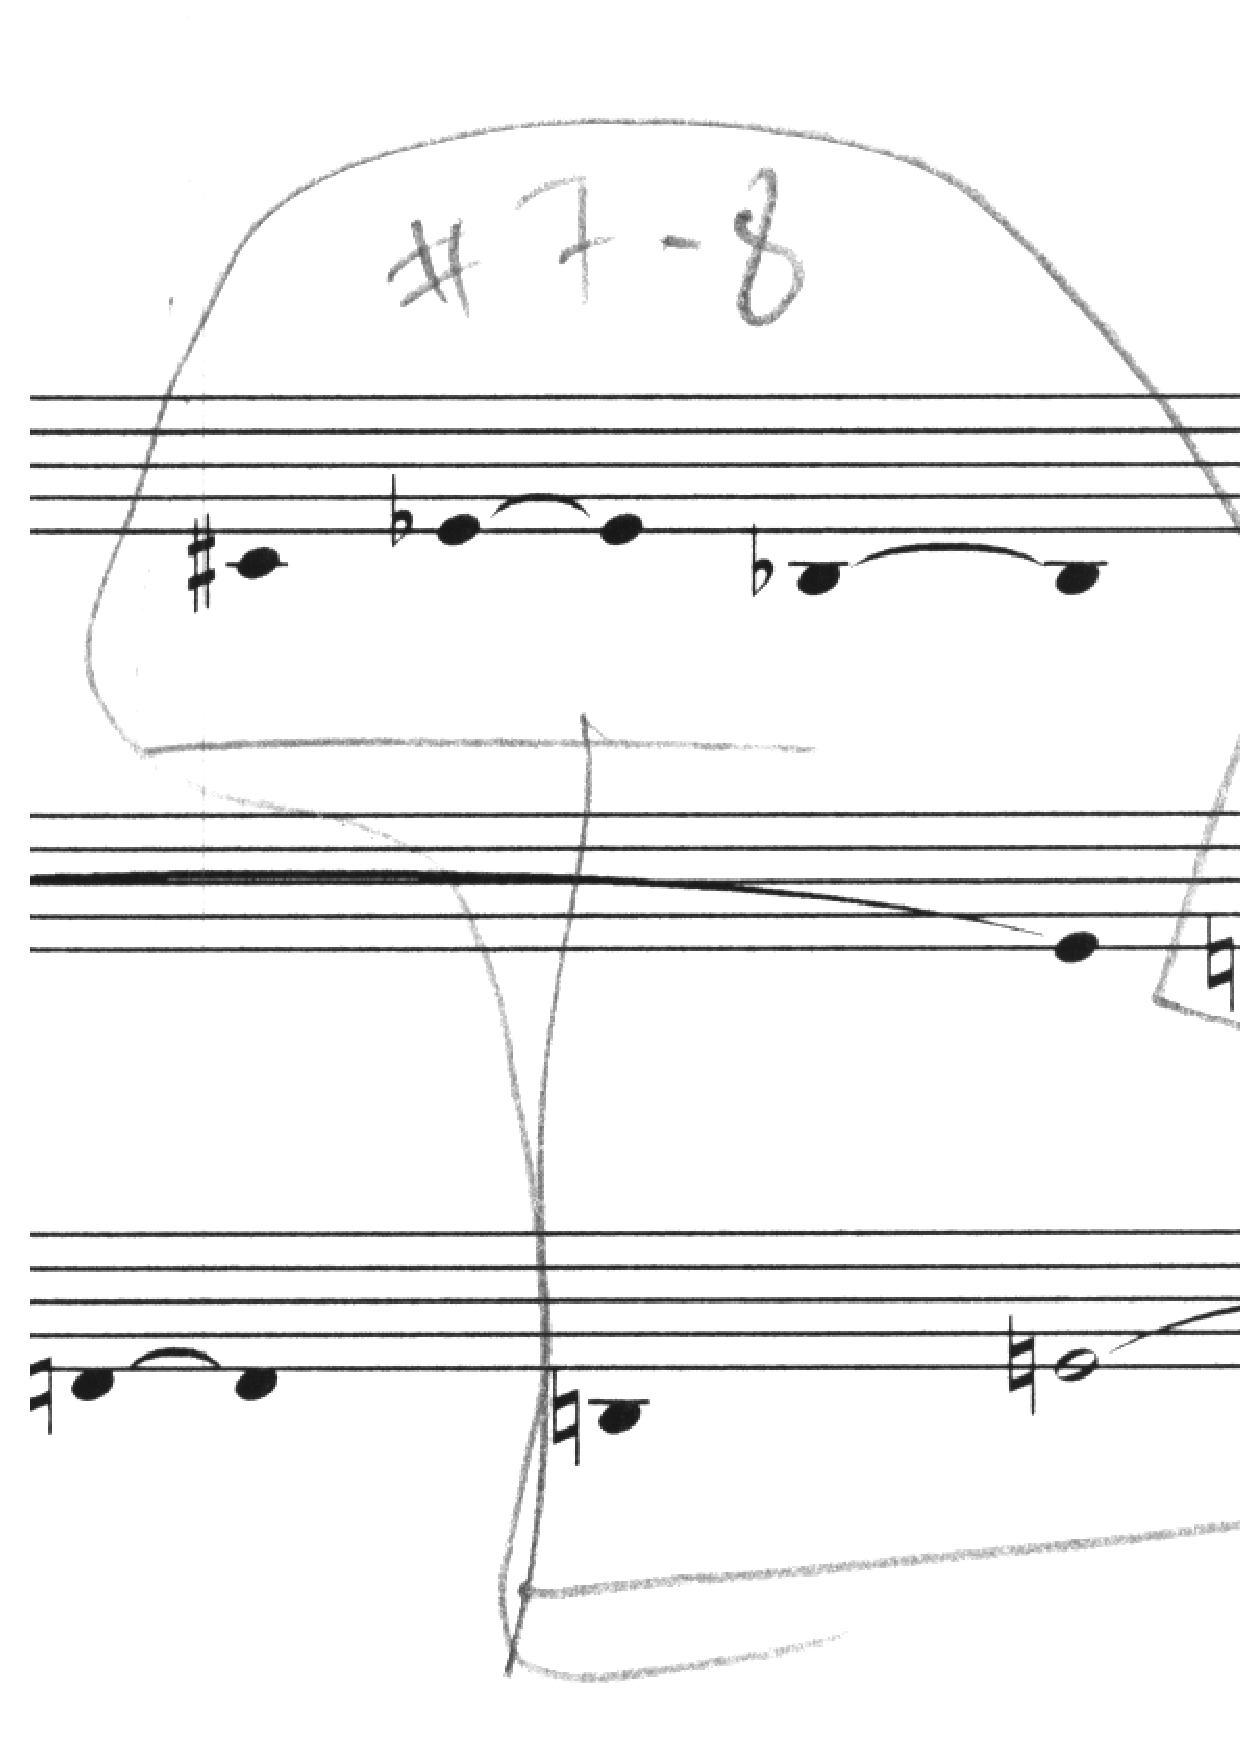
\includegraphics[width=0.75\linewidth]{img/SixTones-transcription-1}
  \end{center}
  \caption{The sketch used for the improvisations for the Six Tones}
\label{fig:sixtones-transcription}
\end{figure}
%\end{wrapfigure}

Apart from being artistically unsatisfying, writing a score to bring to these first meetings with the intention of having it performed `truthfully' would be futile. The chosen method, to improvise from sketches, gave us---all four of us---the opportunity to define our own \emph{subculture} (see \hyperref[sec:1-par:4]{section \ref*{sec:1-par:4}}) against which we could understand the possibilities and the limitations of our collaboration. For the formation of Stefan's and mine subculture, and for our collaboration at large, \emph{The Six Tones} had a great impact, particularly in the social dimension. Thanks to our project with Thuy and My, our process of `tuning-in' had an early start and thanks to it we were given additional opportunities to travel and work together. The importance of the social dimension should not be underestimated: When the construction of musical content is laid out in the open, mediated by a collaboration, the receptiveness of the social relation is paramount.

\emph{The Six Tones} was also important to \emph{Repetition} in the exchange of musical ideas between the two pieces. The sketches we used as a starting-point for our improvisations made use of the same material I had worked out for \emph{Repetition}, though, at the time the \emph{Repetition}-material consisted merely of a tone series in different permutations. For our session I had written out one of these permutations as a monophonic melody line laid out between the three string instruments as if it was one instrument playing (see \hyperref[fig:sixtones-transcription]{Figure~\ref*{fig:sixtones-transcription}}). A number of musical ideas from these sessions (altogether we met four times in May 2006) had a tremendous influence on how the ideas for \emph{Repetition} evolved and how the material was composed.
\begin{itemize}
\item Prior to the Six Tones sessions the idea was to write for six-stringed guitar but the register and the possibilities for alternative tunings persuaded Stefan and me to choose the ten-string guitar instead. 
\item One of the sections of \emph{Repetition} is a transcription of one of the improvisations on the sketch brought to the session on May 17.
\item The scordatura used in \emph{Repetition} was developed according to the   needs presented by the Six Tones project.
\item Some of the sound files used in the first version of \emph{Repetition}   used samples recorded during the Six Tones sessions. 
\end{itemize}  
But there was also a flow of ideas going the other way, from \emph{Repetition} to \emph{The Six Tones} as material composed for the guitar piece was transcribed and used in the ensemble piece.

\section{The first version}
\label{sec:negotiating-3}

\begin{wrapfigure}{r}{0.45\linewidth}
  \begin{minipage}[h]{\linewidth}
    \begin{flushright}
      \musicannot{Repetition Repeats all other Repetitions\\
        \emph{for ten-stringed guitar and computer}\\
        Composed \& premiered in 2006\\
        Commissioned by and dedicated to Stefan \"{O}stersj\"{o}}
    \end{flushright}
  \end{minipage}
\end{wrapfigure}

%%% Local Variables: 
%%% mode: latex
%%% TeX-master: "../ImprovisationComputersInteraction"
%%% End: 

With regard to the background for \emph{Repetition} yet another aspect should be mentioned: its intertextual relation with \emph{Toccata Orpheus} by German composer Rolf Riehm. I became acquainted with \emph{Toccata Orpheus} when Stefan and I participated in the workshop \emph{Knowledge Lab} in Berlin in June 2005. Stefan performed the piece (composed in 1990 for six-stringed guitar solo) and discussed its artistic and interpretative implications in the workshop. Following this event we repeatedly discussed Stefan's idea of making a multimedia performance of \emph{Toccata Orpheus}---i.e. a staging of the piece to allow for a broader expression and a shift of focus to the physicality of the piece. This performance version would involve a sound-scape by me and, during the process of discussing \emph{Toccata Orpheus} and a possible soundscape, we recorded the piece in its entirety as well as details of it for me to use as samples in the sound-scape. We also made a video recording of it that I edited and I started elaborating on the idea of using this material for an electro-acoustic piece with video, addition to the sound-scape. Though introverted in its expression, \emph{Toccata Orpheus} is a highly visual piece as the many different and unusual playing techniques have become part of its construction: there is as much to look at as there is to listen to. Hence, when I started working on the score for \emph{Repetition} in August 2006 the Riehm piece was most certainly a source of inspiration, because I had so closely studied it and discussed its possible performances with Stefan over a long period of time and because I was inspired by the dramaturgy involved in the performance of the piece. In \emph{Toccata Orpheus} the more radical and strained the movement required of the performer the lesser the sound---in itself an interesting reversal of force. In preparation for the sound-scape mentioned above I had made an analysis of the piece based on the movement required to perform each sound, and classified the phrases according to this analysis. The way I decided to approach \emph{Repetition} was very similar: I borrowed Stefan's ten-stringed guitar and constructed a set of sounds based on different playing techniques, some of which are part of contemporary guitar technique and some of which I invented.

\label{sec:3-par:2}
As mentioned above, the raw material for the piece was a simple tone series, a version of an infinitely self-repeating series common to much of Danish composer Per N{\o}rg{\aa}rd's music. Conceptually the piece consists of three permutations of the same raw material, labelled \emph{A}, \emph{B} and \emph{C}. These three motives, distinct both sonically and expressively, are, in a manner of speaking, telling the same story in three different ways. Though it is only possible for the guitarist to play one of these motives at a time, irregularly moving back and forth between them, with the help of the computer part---also made up of three corresponding materials---she or he could create the illusion that all three `stories' are told simultaneously. The guitar and the computer merely `give light' or resonate with one version of the story at a time. The intention was to let the order of the fragments belonging to the three motives be the result of decisions made in performance. In other words, the score consisted of a collection of composed fragments pertaining to one of the three motives and it would be up to the performer to choose the order and the number of repetitions each fragment would play. The interactive challenge, i.e. the question of how to get the computer to `perform' with Stefan without the order, or form, of the music being known in advance, had been factored in already from the start of the our collaboration. \emph{Repetition} was thought to be a testbed for my analysis \index{software}software \emph{timbreMap}, which is a self organising feature map that when fully trained may automatically detect timbral differences in the input audio signal. The idea was to have the \index{software}software `listen' to Stefan and be able to detect when he moved from playing, say, a fragment of the \emph{A} material to some \emph{B} or \emph{C} material. For this reason too it was necessary for me to compose the three materials in such a way that they would be sufficiently timbrally distinct from each other for the \index{software}software to detect the change. At this time, in August 2006, I had a proof-of-concept version of \emph{timbreMap} working which gave me a chance to evaluate and test the different playing styles and their effect on the `listening' computer.

\label{sec:3-par:3}
Though the technique, i.e. the \emph{timbreMap} \index{software}software as interface, may well have worked for the first performances in 2006, we soon realised that for practical reasons with a paper score it would be impossible to employ the level of freedom intended. The six-page score would have to be entirely visible throughout the piece for Stefan to be able to move freely from motive to motive and from fragment to fragment. Though it is possible to set the score up on six music stands it would not be possible to read it.\footnote{In classical guitar technique the guitarist is sitting down, and though in some music it might be possible for the guitarist to move around (most certainly in all other genres), the alternate playing techniques used in this piece make it impossible to play without sitting down.} The solution we chose was to move the decisions concerning the large-scale form of the piece to the pre-performance phase. Stefan would simply work out his version in \index{real-time}\index{time!real-time}non-real-time, and together, following Stefan's instructions, we made a performance version of the score. With time being short and the first performance quickly approaching we also decided to make the interaction between Stefan and the electronic part in this version governed by a foot pedal. Stefan could simply trigger sound-files stored on the computer by pressing a foot switch. This version is still interactive to a certain extent but it is so only if you do \emph{not} consider what the intention had been. How could the original intentions of the piece be `given up' so easily? Neither I nor Stefan saw this first version of \emph{Repetition} as anything other than one possible `version' out of many to come. This agreement was the first step towards the notion of a `\useGlosentry{glos:work_in_movement}{work-in-movement}'\footnote{The term `work-in-movement' was coined by Umberto Eco to distinguish a particular species of `open works' in which ``the auditor is required to do some of this organizing and structuring of the musical discourse. He collaborates with the composer in making the composition''. In the case of \emph{Repetition} the `auditor' is replaced by the performer but that is also the case in the examples of work-in-movements that Eco provides. \cite{eco68}.} and by limiting the openness in this particular instance we greatly increased the future possibility for openness. This expanded concept of openness or work-in-movement---whereby each instance could not only choose its form in the course of the performance, but alter its interaction scheme, its instrumentation, its score, and so forth---was not originally specified by me. If Peter Kivy is right in suggesting that \emph{discovery} is what best describes the activity of composers,\footcite[214]{kivy02} then we were truly composing when we impeded \index{real-time}\index{time!real-time}real-time choice in the first version of \emph{Repetition} because, in this and other choices we made, its potential as a `work-in-movement' was \emph{discovered}.

%%
%\hspace{0.5\linewidth}
\begin{wrapfigure}{r}{0.5\linewidth}
  \begin{minipage}[H]{1\linewidth}
    \advance\rightskip-1cm
     \vspace{0.5cm}\label{fig:inlay2}
\musicannot{
Marcel Duchamp, introduced the notion of the ``personal 'art coefficient' '' in a discussion concerning the creative act. Specifically Duchamp was referring to the immanent processes, those in which the artist alone is involved and which ultimately lead to ``art in the raw state---\`{a} l'\'{e}tat brut'' and, in short, it constitutes the difference between the artistic intention and its realization. The gap goes unnoticed by the artist and it represents his (or her) inability ``to express fully his intention''\footcite{duchamps57} Duchamp concludes that ``the personal 'art coefficient' is like an arithmetical relation between the unexpressed but intended and the unintentionally expressed.''\footcite{duchamps57} It is primarily the description of the art coefficient as a \emph{relation} that I find interesting. What could the `interaction coefficient' constitute? The notion of the ``unintentionally expressed'' as having a relation to the ``unexpressed but intended'' could be directly transferred to interaction: In any interaction there are unintended outcomes (\emph{Why did the computer go down?} or \emph{Why did you sound so angry?}) as well as intended but tacit (\emph{How come the computer doesn't understand what I want to do?}). What can the interaction coefficient tell us about an interaction? What, if the interaction is part of an artistic context, what would the relation between the art coefficient and the interaction coefficient be? Would they be the same or different?
}
  \end{minipage}
\end{wrapfigure}
%%% Local Variables: 
%%% mode: latex
%%% TeX-master: "../ImprovisationComputersInteraction"
%%% End: 

%%
\label{sec:3-par:4}
Another reason we allowed ourselves to change the scheme of the piece, and to continue to do so, was the fact that in the rehearsals it was obvious the alterations had worked out really well. Not only was the new form convincing, the integration between the electronics and the guitar was seamless. Despite the lack of performer-computer interactivity, several listeners in the audience for the first performances commented that the piece sounded like it was interactive (i.e. interactive in the sense I had intended it to be). Some even thought it was and were surprised to learn about its relatively static set-up. The sounds I used for the electronic part were samples from the improvisations we did with \emph{The Six Tones} (see \hyperref[sec:negotiating-2]{Section~\ref{sec:negotiating-2}}) as well as samples I had from playing Stefan's ten-stringed guitar when composing the score for \emph{Repetition}. Could it be that the interaction in the production phase of \emph{Repetition} substituted for the \index{real-time}\index{time!real-time}real-time interaction in the performance? This would imply that interactivity is a quality that `objects' can absorb or occupy, that they can pick up and then adhere to, independent of time. The interaction between Stefan and me, and between us and Thuy and My (in the project \emph{\useGlosentry{glos:six-tones}{The Six Tones}}), was encoded in the sound-files used for the computer part and in the music as performed. Certainly a pleasing thought, though I doubt the reason for the deceptive impression of performer-computer interactivity in this version of \emph{Repetition} is directly related to interaction of a different kind and in a different time (although interactivity does not necessarily have to be \index{real-time}\index{time!real-time}real-time as discussed in \hyperref[sec:time-interaction]{Section \ref*{sec:time-interaction}}) but I believe that, in musical practice, interaction of the kind Stefan and I were engaged in whilst preparing for these first performances is a factor (a coefficient?) that positively influences the chances for a successful result---where `successful' is defined as `all participants are generally pleased with the outcome'. It is this coefficient that creates the illusion of performer-\index{interaction!computer}computer interaction.


\section{Symphonie Diagonale}
\label{sec:negotiating-4}

\begin{wrapfigure}{r}{0.5\linewidth}
  \begin{minipage}[h]{\linewidth}
    \begin{flushright}
      \musicannot{
        Repetition Repeats all other Repetitions, Symphonie Diagonale\\
        \emph{for ten-stringed guitar, computer and video projection}\\
        Composed \& premiered in 2007\\
        Prepared in collaboration with Stefan \"{O}stersj\"{o}}
    \end{flushright}
  \end{minipage}
\end{wrapfigure}

%%% Local Variables: 
%%% mode: latex
%%% TeX-master: "../ImprovisationComputersInteraction"
%%% End: 

The  motivation for the second version we did, the combination of \emph{Repetition} and \emph{Symphonie Diagonale},\footnote{The silent movie \emph{Symphonie Diagonale} is an eigth-minute modernist film classic by the Swedish artist Viking Eggeling dating from 1924.} was to use the film as a springboard for the making of a radically different version of the guitar and electronics piece. By itself, the idea of combining two totally unrelated works, separated in time by 83 years and created in different media, is extremely odd but the first version of \emph{Repetition} had already been performed four times and it was at this point scheduled for another four performances. Though the potential for \emph{Repetition} as a work-in-movement had been discovered, its status as such had not yet been established and, owing to the `success' of the first version, we had to resist the comfortable notion of staying with the first version. Hence there was a need for a second version as different from the previous one as possible. 

\label{sec:4-par:2}
This version is even less interactive than the first in that its performance version is static: the film, along with the electronic track, is played back and Stefan is solely responsible for keeping the synchronisation tight between the film and the electronics on the one hand, and the guitar part on the other. The binary control interface is now reduced to constitute zero or one: the video is either playing or it is not. Again, we have to see the bigger picture and look at the processes that proceeded the performances of the second version.\footnote{The process of constructing this version is described in some detail in \cite{ostersjo08}.}

\begin{wrapfigure}{l}{0.2\linewidth}
  \begin{center}
    
\includegraphics{img/eggeling-25}
  \end{center}
    \caption{Symphonie Diagonale}
    \label{fig:eggeling-25}
 \end{wrapfigure}
\label{sec:4-par:3}
If for the first version there was a relatively clear distinction between my tasks (providing the raw material, the score and the sounds) and Stefan's (constructing a performable version of the piece out of the components I gave him), our interactions for this version were less defined. After an initial analysis of the film, an obviously black and white eight-minute abstract film---white graphical shapes, evocative of paper cut-outs, on black background (see \hyperref[fig:eggeling-25]{Figure \ref*{fig:eggeling-25}})---we started mapping the musical material onto the imagery. We were working with a recording of the guitar part, and many of the phrases fitted the rhythm of the film without alteration: we were inspired by the lack of resistance of the undertaking and the version was completed in a few days. 

\label{sec:4-par:4}
The work we did on those days in January 2007 involved a great many artistic choices that were all made by continuous negotiation between `performer' and `composer' with an almost complete merging of the two agents into one \emph{musician}. Neither of the agents seemed to have the interpretative precedence and, to use the terminology from \autoref{sec:1-par:3}, the \emph{\useGlosentry{glos:poietic}{poietic}} and \emph{\useGlosentry{glos:esthesic}{esthesic}} domains overlap and interact in a recursive fashion. Again, the interactivity in the performance WAS supplemented by interactivity in the construction. Although, as I pointed out above, the main purpose of this version was to create a breach that would allow us to move on to yet another version of \emph{Repetition}, the film component added an extra constraint: if we wanted to stay faithful to the film, i.e. not alter it in any significant way, then the non-interactive, static rather than dynamic version we ended up with was almost our only option. Why then did we not alter the film? It is perfectly possible to take \emph{Symphonie Diagonale} and cut it up into small fragments that get triggered by the guitar or by the audience or by any other factor. In the making of this version, the film was the method, rather than the result, the intended result of which was to further open up the work \emph{Repetition}. In that sense this version was an intermediary between the first version and any succeeding ones.

\label{sec:4-par:5}
At this point, after the \emph{Symphonie Diagonale} version had been performed it started to become clear that \emph{Repetition} had in it an infinite number of \emph{Repetitions}. Its `authenticity' lies in the collaborative aspects of its production `versioning'\footnote{\index{software}Software versioning, also known as revision control, is used to differentiate between different editions or `releases' of e.g. software.} rather than its detailed specifications. Its material work identifying instructions---in this case the scores, the samples and sound-files, the recordings of prior performances; everything belonging to its prior versions---could be picked up by any two or more musicians willing to engage in the construction of another version (in the sense of construct rather than construe).

\section{Collaborative music}
\label{sec:negotiating-5}
Collaborative artistic work in general may be seen as a reaction against the singularity of the romantic as well as modernist view of the artist as the inspired, predominantly white male creator from whom great artworks emanate. It is, however, very difficult to draw a distinction between collaborative work as decentralised division of labour on the one hand and, let us call it, less collaborative work that stems from centralised authority on the other. To begin with, in music, it is difficult to imagine a performance that does not involve collaboration between different agencies at some level of the production. Perhaps the \emph{Study No. 21, Canon X}\footnote{Studies No. 4 through 30 were composed between 1948 and 1960.} from \emph{Studies for Player Piano} by American composer Conlon Nancarrow can serve as an example of `less-collaborative' music. Not only was it composed for a mechanical instrument\footnote{Like so much of Nancarrow's other music, \emph{Study No. 21} is written for a player piano, the Ampico player piano to be specific (see \url{http://en.wikipedia.org/wiki/Player_piano} for more information on these instruments).} and punched into the player roll rather than written out in traditional notation, it was not performed in public (with one exception) until after Nancarrow's international breakthrough in 1982. The following is an excerpt from an interview with Nancarrow by William Duckworth that gives evidence of the seclusion and non-collaborative environment in which this and the other Studies were composed:
\begin{squote}
  \emph{Duckworth}: Between the early 1940s and 1960, when you were writing most of your Studies, was anyone hearing your music besides you?\\
  \emph{Nancarrow}: No.\\
  \emph{Duckworth}: Were you just playing them for yourself?\\
  \emph{Nancarrow}: Occasionally someone would hear it, but very
  occasionally. \footcite[49]{duckworth99}
\end{squote}

\label{sec:5-par:2}
At the other end of the collaborative/non-collaborative continuum, we could place any example of free jazz group improvisation in which nothing is pre-determined apart from the instruments, the players and the physical (and usually social) context. Evan Parker writes about a recording of a trio improvisation featuring, apart from himself on saxophone, Derek Bailey and Han Bennink: ``We operate without rules (pre-composed material) or well-defined codes of behavior (fixed tempi, tonalities, serial structures, etc.) and yet are able to distinguish success from failure''.\footcite[As cited in][39]{lebaron02} A lack or dismissal of ``rules'' of operation or ``codes of behavior'' is not necessarily a prerequisite for collaboration but may be seen as a method by which the participants are forced to collaborate in order to avoid cacophony and chaos. (Though, admittedly, chaos may also be a most viable means of collaborative expression.) 

\label{sec:5-par:3}
A different beam of collaborative music (forced collaboration?), orthogonal to the Nancarrow-Parker axis, can be found in the brilliant and skilful output of John Oswald, who coined the term `Plunderphonics' for a ``retro-fitted music, where collective melodic memories of the familiar are minced and rehabilitated to a new life''.\footcite[Oswald quoted in][49]{lebaron02} By cutting up recordings of popular music into small chunks and pasting them together in unexpected combinations he created a schizophrenic music---perhaps the very epitome of postmodern music---in which seemingly random collections of snippets of sound are forced to collaborate.\footnote{Recommended listening is the 1'46'' long \emph{Cyfer} on the CD \emph{Plexure}: \cite{plexure93}} Although the artists whose music he reorganised rarely agreed to the refactoring,\footnote{Based on Michael Jackson's song ``Bad'' Oswald's collage ``DAB'' from the 1995 CD \emph{Plunderphonics} caused a copyright debate with legal consequences more than a decade before peer-to-peer sharing and illegal downloading. CBS Records, Michael Jackson and the Canadian Recording Industry Association claimed that Oswald's work was illegal and demanded that the recordings of his work be destroyed. \cite[See][]{wired95}.} Oswald, in a manner of speaking, set up a distant collaboration with them and with the context they belonged to, comparable to Marcel Duchamp's readymades. On the opposite side to Oswald, but on the same axis, we could place any kind of \useGlosentry{glos:fixed_media}{fixed media}, electro-acoustic so-called `tape piece' (i.e. studio produced music played back in concert on speakers), such as John Chowning's \emph{Stria}, in which all sound material used is synthesised (as opposed to sampled real-world sounds.

\label{sec:5-par:4}
These are examples of regions of musical collaboration in a multiaxial space of musical practice. As mentioned above, some degree of collaboration is likely to play a part in any music and, as a consequence, it may be suggested that `collaborative', when used to describe the coming into existence of a musical work, is too unspecific. If so, how may the multiple, collaborative, \useGlosentry{glos:poietic}{poietic} processes of \emph{Repetition} be described? That `work-in-movement' may be used to define the work type it belongs to is of little help; it only tells us that we are dealing with an unfixed work and that it needs involvement of others apart from the composer to be instantiated, but not what the nature of the collaboration constitutes. Depending on the version we are examining, \emph{Repetition} as a `work-in-movement' will inevitably move between many different locations in the collaborative space proposed above. Looking back at the phase at which the work revealed its possibilities for openness (\hyperref[sec:4-par:5]{see the last paragraph of \ref{sec:negotiating-4}}) we may conclude that collaboration constitutes the ontological essence of the work: it is a work whose identity is to be found in the interactions that has preceded its productions rather than in its instructions. The collaborative aspect of \emph{Repetition} is the work.


% Although most musical activities involve collaboration of some kind, in \emph{Repetition} collaboration is the very essence of the work.

% the particular kind of collaboration that evolved while working on \emph{Repetition} may be distinguished in that it constitutes the very essence of the work.

%  it is perhaps possible to distinguish the kind of collaboration identified with \emph{Repetition} from the range of collaborative activities that make part of most musical activity in that the collaborative aspect in \emph{Repetition} has been made its essence.

%%%%%%%%%%%%%%%%%%%%%%%%%%%%%%%%%%%%%%%%%%%%%%%%%%%%%%%%%%%%%%%%%%%%%%%%%%%%%%%%
\section{The annotated score}
\label{sec:negotiating-6}
%%%%%%%%%%%%%%%%%%%%%%%%%%%%%%%%%%%%%%%%%%%%%%%%%%%%%%%%%%%%%%%%%%%%%%%%%%%%%%%%

\emph{Repetition} was conceived prior to its preparatory studies and the experiences gained from its first and second versions as an open work similar to some of my other works like \hyperref[sec:drive-2003]{\emph{Drive}}. It was manifested as building blocks notated and left to the performer to organise them: a fairly traditional example of `open work'. The way the process has evolved, however, informed by the knowledge produced in the study performed on Stefan and Love Mangs (\hyperref[sec:negotiating-1]{see Section \ref*{sec:negotiating-1}} and \ref*{sec:negot-music-work}), the emphasis in the term `work-in-movement' has travelled from `work' to `movement', and the emphasis on the `composer' in the quote from Eco\footnote{``The auditor is required to do some of this organizing and structuring of the musical discourse. He collaborates with the composer in making the
composition.'' \cite{eco68} The auditor is interchangeable but not the composer.} should in our case instead be put on `collaborate', because the action is more important than the subject. Altogether, we have  travelled quite a long way from Eco's original notion which, to begin with, by the `auditor' implies a (passive) `receiver' rather than a collaborator. The `work-in-movement'  implied here is a literal construction kit, to be assembled and re-assembled in a recursive process that should be allowed to continue outside the collaboration that gave rise to it. Stefan and I set it in motion but its authenticity can only be derived from the continuous movement, an open-source music that may be dismantled and reconstructed, added to and altered, according to its conglomerate of participants.

In order to realise fully the notion of a work-in-movement, the process of documentation, or in musical notation terminology the work identifying instructions, needs to be reconsidered. The way \emph{Repetition} as a work has evolved, a traditional printed score in musical notation, no matter how detailed the written instructions are, would be misleading. As has already been pointed out, the operative word in `work-in-movement' is precisely the movement: the change, the difference that makes a difference. Therefore the score will need to communicate the process rather than the result, in itself not a novel idea. The musical notation will no doubt constitute an important part of the documentation but it will not be sufficient in itself.

As discussed, apart from this more, let us call it musicological, aspect of the notation of \emph{Repetition}, there are also practical issues regarding the notation and the score that need to be resolved in order to allow for the work to continue to evolve. If the performer is to be able to alter the order of the sections according to choices made in performance, the score needs to be adopted. If, however, the performer chooses to do what Stefan did in the first version, i.e. settle on a form prior to performance, the `final' score should easily allow for this. Finally, adding the third version discussed above---with a real-time interactive computer part---to the list of possible modes of performance, the score needs to fully document and guide the performer in how to set up the computer part. 
\begin{figure}[htb]
  \centering
  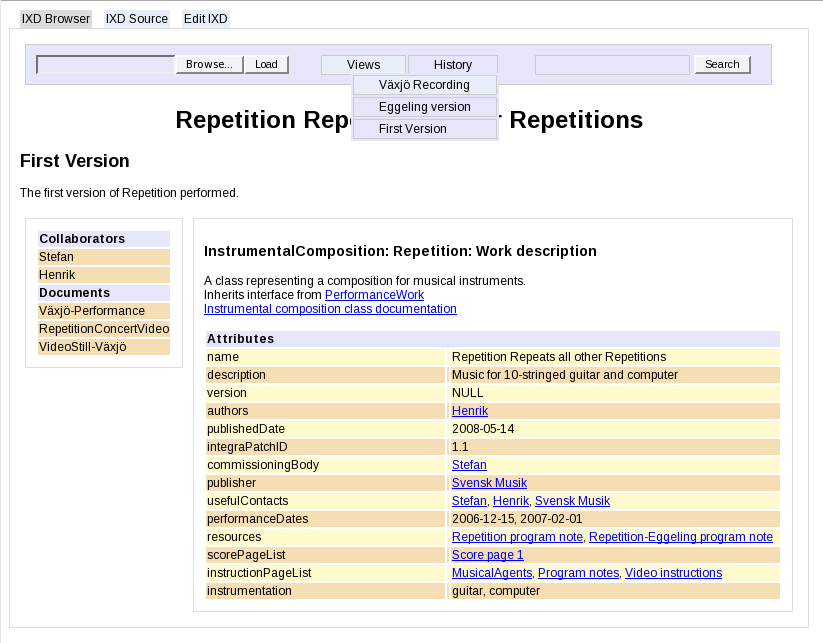
\includegraphics[width=\linewidth]{img/Work.png}
  \caption[The IntegraBrowser: base record.]{The IntegraBrowser displaying the base record for \emph{Repetition Repeats all other Repetitions}.}
  \label{fig:ib-1}
\end{figure}

\begin{wrapfigure}{r}{0.4\linewidth}
  \begin{minipage}[h]{\linewidth}
    \begin{flushright}
      \musicannot{IntegraBrowser\\
        \emph{Offline browser for the Integra XML\\documentation format.}}
    \end{flushright}
  \end{minipage}
\end{wrapfigure}

%%% Local Variables: 
%%% mode: latex
%%% TeX-master: "../ImprovisationComputersInteraction"
%%% End: 

To allow for these considerations---the performance aspect and the `work-in-movement' aspect---I have developed an experimental web application\footnote{A Web application is a piece of software that is run in a standard web browser.}. This application is an attempt at allowing for what may be termed the `annotated score', an information source relating to a piece of music (or any other kind of art work) that may hold a score and any number of other documents referring to the piece (an audio or video recording, a performance instruction, text instruction, information on previous `instances', etc., all of which may be interlinked). With the Web application, called the Integra Browser, such collections of heterogeneous data pertaining to \emph{Repetition}, or any other piece of music or general art work, may be browsed and edited (see the screenshots provided in Figure \ref{fig:ib-1}, \ref{fig:ib-2} and \ref{fig:ib-3}). The design considerations set up for the annotated score were that
\begin{itemize}
\item It should encourage the interpreter to engage in a collaborative
  process similar to the one we have gone through with the primary
  goal of not repeating or recreateing our process but to find his or her
  own unique version.  
\item It should allow the performer to look up any part of the
  notation at any time.
\item It should allow for the interpreter to easily create a static
  form that s/he can use in performance.
\item It should contain all the \index{software}software and all the sound-files needed
  to create an interactive as well as a non-interactive version of the
  computer part.
\item It should document important parts of our collaboration and
  allow for other performers to add important parts of their own
  collaborations to the work.
\end{itemize}
Realising the first versions of the notion of an annotated score and fulfilling these design goals is possible by making use of the \emph{libIntegra} framework and the associated IXD file format.\footnote{The details of the format is described in \cite{frisk-bull07}. See also \cite{frisk-bullock08}}

\begin{figure}[htb]
  \centering
  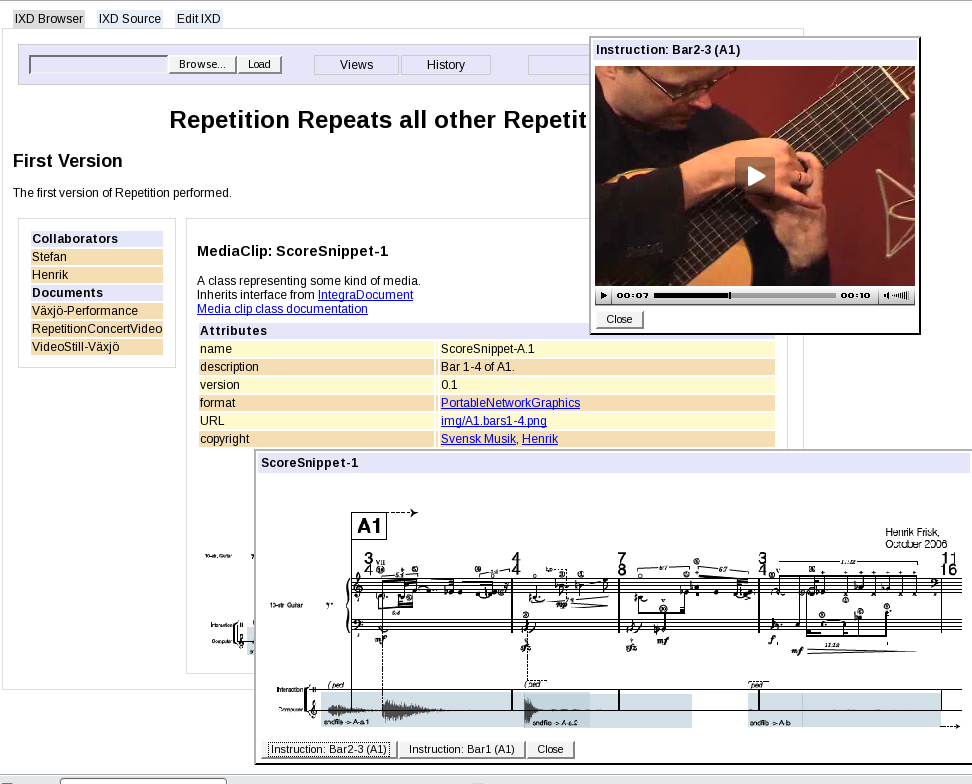
\includegraphics[width=\linewidth]{img/Score.png}
  \caption[The IntegraBrowser: an instruction video.]{A second pane displaying a score snippet with an associated instruction video.}
  \label{fig:ib-2}
\end{figure}

\begin{figure}[htb]
  \centering
  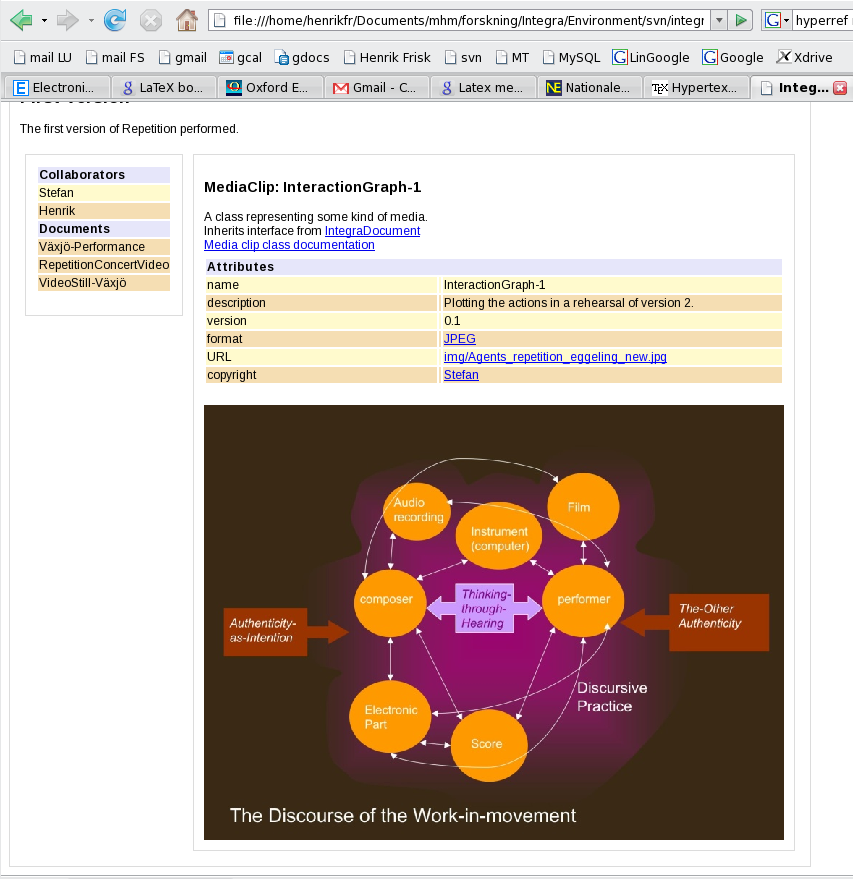
\includegraphics[width=\linewidth]{img/Discourse.png}
  \caption[The IntegraBrowser: meta-information.]{This panel shows how meta-information and different modes of analysis may be attached to a score. This picture is mapping the interactions between the different agents in my collaboration with Stefan \"{O}stersj\"{o}.}
\label{fig:ib-3}  
\end{figure}

\section{Summary}
\label{sec:summary-2}

In this chapter I have tried to unwrap the process that led to the work-in-movement \emph{Repetition Repeats all other Repetitions} and the significance of the pre-study phase in which Stefan and I attempted a closer understanding of the musical collaboration as method. These studies provided important information that shaped how the project evolved. \useGlosentry{glos:six-tones}{The Six Tones} (working on the piece as well as working with the group) and the experiences gained from working with Vietnamese music in general further deepened the collaborative aspect of the project which neither one of us had yet fully conceived of as the open work type that had begun to emerge. The first performance version deviated from almost all aspects of the intention of the piece and for the same reason provided us with an opening towards a different understanding of open form. Therefore, the collaboration did not end with the first performance, rather, it had just started. The need to break loose from that version gave birth to the idea of a version for the abstract dadaist film \citetitle{eggeling24} by \citeauthor{eggeling24}. Again, this version took us further away from the original intentions but closer to the new intention: the concept of the work-in-movement. A short overview of music and collaboration, and some possible points along the collaborative/non-collaborative continuum were presented. Finally, the augmented score as a carrier of a work-in-motion was proposed. An experimental version of a Browser for augmented scores built on top of the Integra framework and file format was presented. 

It is my hope that \emph{Repetition} will not come to a halt but continue to develop. Versions for other (string) instruments are possible, but also versions for computer(s) only. A work-in-movement thrives on its motion and must not stagnate.
\newpage
\thispagestyle{empty}
%%% Local Variables: 
%%% mode: latex
%%% TeX-master: "../ImprovisationComputersInteraction"
%%% End: 